	\begin{figure}[tbh]
		\centering
		\begin{minipage}[t]{0.24\textwidth}
		\centering
		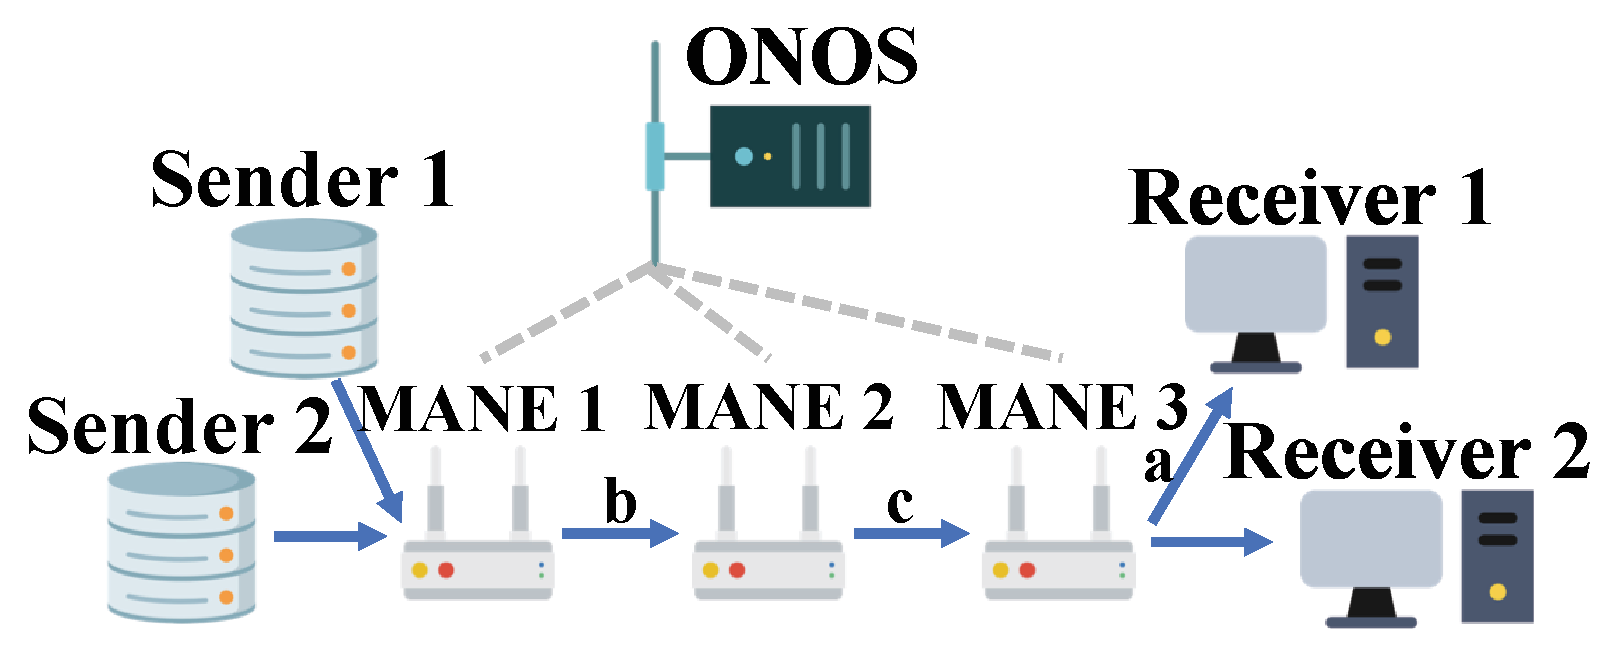
\includegraphics[width=\textwidth]{fig/scenario_2.eps}
		\caption{Mininet testbed topology (scenarios 1 and 2).}
		\label{scenario_2} 
		\end{minipage}
		\hfill\begin{minipage}[t]{0.23\textwidth}
		\centering
		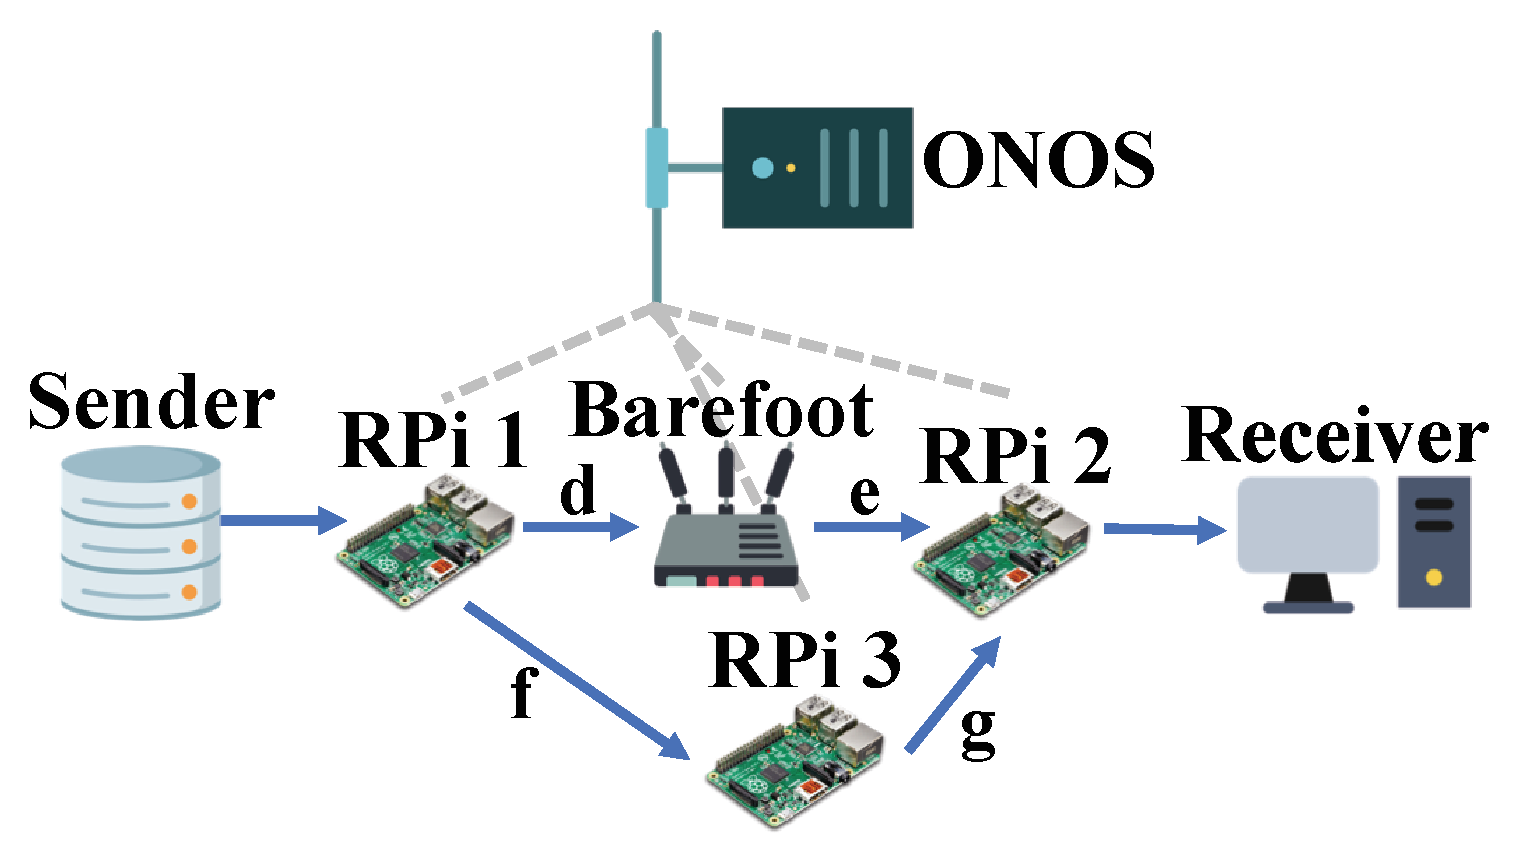
\includegraphics[width=\textwidth]{fig/scenario_3.eps}
		\caption{Real testbed topology (scenario 3).}
		\label{scenario_3} 
		\end{minipage}
\vspace{-0.1cm}
	\end{figure}

\section{Demonstration Setup} \label{sec:setup}
\begin{comment}
We use real H.264/SVC video sequences in our demonstrations. 
We develop three scenarios, where
the first
two scenarios are done in mininet with software MANEs (running the reference P4 software switch, called {\em bmv2}~\cite{bmv2}) and virtual hosts.
We deploy real MANEs: a Barefoot switch and three
Raspberry Pi ones (with bmv2) in the last scenario, in order to show the practicality of our prototype system. 
We describe the three scenarios below:
\begin{itemize}
	\item {\bf Intelligent packet drops of a single video stream.}
	We construct a simple network with a sender, a controller, a MANE, and a receiver. The network is similar to Fig.~\ref{scenario_2} but with only a pair of sender/receiver and a MANE. The mininet bandwidth on the link is varied over time by scripts. In the MANE, we implement tail, EL, and RDO logics, and compare their performance. 
	
	\item {\bf Optimal packet drops across multiple video streams.}
	We construct a network with two pairs of senders and receivers, and three MANEs, as shown in Fig.~\ref{scenario_2}. We vary the bandwidth of link $c$ over time. MANE 2 determines which packets to drop to maximize the overall quality. Moreover, MANE 2 notifies MANE 1 to drop the packets (early) to avoid bandwidth wastes on link $b$. We evaluate different packet-discarding logics and video sequences.  


	\item {\bf Error resilience with real P4 switches.}
	The network we construct includes a sender, a controller, one Barefoot switch, three Raspberry Pi switches (with bmv2), and a receiver, as revealed in Fig.~\ref{scenario_3}. All the links are Fast Ethernet cables. The bandwidths of links $d$ and $e$ are higher than the bandwidths of links $f$ and $g$. We physically remove link $e$ during streaming, and we expect to see that the ONOS controller reroutes the video stream through the Raspberry Pi 3 at the bottom. Because we configure links  $f$ and $g$ to have lower bandwidth, the video quality goes down. When we plug the Ethernet cable back, the ONOS controller reroutes the video stream over the Barefoot switch, and the quality of video stream goes up. 

\end{itemize}

%{\bf Preliminary evaluation.}
%To evaluate the performance of RDO, we use the following Quality of %Experience (QoE) measurements to compare tail drop, base-only and RDO %algorithms and compare the RDO with the general switches as well.

%\begin{itemize}
%\item {\bf Network latency}  Since more and more people watch video online, network latency is an important factor that impact users on watching videos.
%\item {\bf Network bandwidth} Videos nowadays usually have large resolutions, especially the presence of 4K videos. However, it is difficult to upgrade the network bandwidth on network links, which are usually fixed. Thus, we evaluate our algorithms and expect RDO can   
%\item {\bf Video quality}
%\end{itemize}

\end{comment}